\documentclass[12pt,a4paper]{article}
\usepackage[utf8]{inputenc}
\usepackage[croatian]{babel} % For Croatian 
\usepackage[T1]{fontenc} % Better hyphenation for wrods with digraphs čćžšđ
\usepackage{graphicx}
\usepackage{color}
\usepackage{float} % For manualy figure postioning
\usepackage{listings} % Support for .txt listings w/o begin{verbatim}
\usepackage[usenames,dvipsnames]{xcolor} % Enabling more defined colors
\usepackage{datetime}
\usepackage{tocloft} % For Toc with dots
\usepackage[left=3cm,top=2.5cm,right=2.5cm,bottom=2.5cm]{geometry} 
\usepackage{fancyhdr} % For fancy headers and footers
\usepackage[nottoc]{tocbibind} % For adding Bilbiography in TOC
\usepackage{amsmath}
% ---------------------------------------------------------------------------
% Fancy header definition
% ---------------------------------------------------------------------------
\setlength{\headheight}{15.2pt}
\pagestyle{fancy}
\fancyhf{}
\rhead{ \bfseries \color{MidnightBlue}  }
\renewcommand{\sectionmark}[1]{\markright{#1}{}} % Section mark to small case
\renewcommand{\subsectionmark}[1]{\markright{#1}{}} % Section mark to small case
\lhead{\sectionmark}
\lhead{\rightmark}
\rfoot{\thepage}
\linespread{1.3}

\renewcommand\lstlistingname{Unos}
\renewcommand\lstlistlistingname{Unos}

\lstnewenvironment{code}[1][]%
  {\minipage{\linewidth} 
   \lstset{
        basicstyle=\ttfamily\footnotesize,
        language=Matlab,
        captionpos=b,
        keywordstyle=\color{blue},
        frame=single,
        #1}}
  {\endminipage}

\definecolor{mygreen}{rgb}{0,0.6,0}
\definecolor{mygray}{rgb}{0.5,0.5,0.5}
\definecolor{mymauve}{rgb}{0.58,0,0.82}

\lstset{ %
  backgroundcolor=\color{white},   % choose the background color; you must add \usepackage{color} or \usepackage{xcolor}
  basicstyle=\footnotesize\ttfamily,% the size of the fonts that are used for the code
  breakatwhitespace=false,         % sets if automatic breaks should only happen at whitespace
  breaklines=true,                 % sets automatic line breaking
  captionpos=b,                    % sets the caption-position to bottom
  commentstyle=\color{mygreen},    % comment style
  deletekeywords={...},            % if you want to delete keywords from the given language
  escapeinside={\%*}{*)},          % if you want to add LaTeX within your code
  extendedchars=true,              % lets you use non-ASCII characters; for 8-bits encodings only, does not work with UTF-8
  frame=single,                    % adds a frame around the code
  keepspaces=true,                 % keeps spaces in text, useful for keeping indentation of code (possibly needs columns=flexible)
  keywordstyle=\color{blue},       % keyword style
  language=C,                      % the language of the code
  morekeywords={*,...},            % if you want to add more keywords to the set
  numbers=left,                    % where to put the line-numbers; possible values are (none, left, right)
  numbersep=5pt,                   % how far the line-numbers are from the code
  numberstyle=\tiny\color{mygray}, % the style that is used for the line-numbers
  rulecolor=\color{black},         % if not set, the frame-color may be changed on line-breaks within not-black text (e.g. comments (green here))
  showspaces=false,                % show spaces everywhere adding particular underscores; it overrides 'showstringspaces'
  showstringspaces=false,          % underline spaces within strings only
  showtabs=false,                  % show tabs within strings adding particular underscores
  stepnumber=2,                    % the step between two line-numbers. If it's 1, each line will be numbered
  stringstyle=\color{mymauve},     % string literal style
  tabsize=2,                       % sets default tabsize to 2 spaces
  title=\lstname                   % show the filename of files included with \lstinputlisting; also try caption instead of title
}

\begin{document}

% Section, figure, table numbering
\renewcommand{\thesection}{\arabic{section}.}
\renewcommand{\thesubsection}{\arabic{section}.\arabic{subsection}}
\renewcommand{\thefigure}{\arabic{section}.\arabic{figure}} 
\renewcommand{\thetable}{\arabic{section}.\arabic{table}}

\newpage
\begin{titlepage}
\begin{center}
% Definition of HRule command
\newcommand{\HRule}[1]{\rule{\linewidth}{#1}}

\textsc{Sveučilište Josipa Jurja Strossmayera u Osijeku}\\[0.2cm]
\textbf{\textsc{Elektrotehnički fakultet Osijek}}\\[4.5cm]
%\includegraphics[scale=0.35]{graphs/etfos_logo.eps}\\[2cm]    

% Title
%\HRule{1.5pt} \\[0.2cm]

{\large \bfseries \textsc{Svalina Marijan, D287} \\ [1 cm] } 
{\LARGE \bfseries \color{MidnightBlue} 
ROBOTSKI VID \\ laboratorijske vježbe \\ [0.5cm] }
{\large \bfseries izvještaj} \\ [0.2cm]

%\HRule{2pt} 

\vfill
% Author 

\begin{minipage}{0.4\textwidth}
\begin{center} \large
Osijek, \today \\
\end{center}


\end{minipage}
\end{center}
\end{titlepage}
\newpage
% Toc  
\renewcommand{\cftsecleader}{\cftdotfill{\cftdotsep}}
\tableofcontents 
% Removing page numbering from TOC
\thispagestyle{empty}

\newpage
\setcounter{page}{1}


\setcounter{figure}{0}
\section{Vježba 1: Uvod u OpenCV i podešavanje radne okoline}

\subsection{Cilj vježbe}
Upoznati se s bibliotekom OpenCV. Podesiti i proučiti alate za
prevođenje i izvršavanje izvornog koda. Napisati jednostavan program za
određivanje rubova na slici pomoću \emph{Canny-evog} detektora rubova.
Proširiti program funkcijom rezanja slike i dodati mogućnosti učitavnja
videa.\\

\subsection{Kratak info o OpenCV-u}

OpenCV (\emph{Open Source Computer Vision Library})je biblioteka C i C++
funkcija koje se često upotrebljavaju u računalnom vidu. Početno
razvijena od strane Intel-a, a trenutno ju održavaju Willow Garage i
Itseez.  Slobodna je za upotrebu pod uvijetima BSD licence. Biblioteka
se izvodi na svim većim platformama. Fokusira se na obradu slike u
stvarnom vremenu.

\subsection{Radna okolina}

\begin{description}
  \item[OS:] Ubuntu 12.04
  \item[Biblioteka:] OpenCV 2.4.6
  \item[Prevodioc:] GCC 4.6.3 
  \item[Ostalo:] pkg-config 0.26
\end{description}

Ubuntu 12.04 je izabran zbog stabilnosti, jednostavnog podešavanja i 
dostupnosti velike količine već priprmljenih programskih paketa.
OpenCV 2.4.6 je zadnja stabilna verzija u trenutnku pisanja. Odabrana
je jer se razvoj aplikacija odrađivao na više računala s različitim 
GNU/Linux distribucijama te zbog dostupnosti najnovih funkicija.
GCC 4.6.3 je zadna verzija koja dolazi s Ubuntu 12.04 distribucijom.
pkg-config alat je korišten jer on automatski izlista potrebne
opencv biblioteke i datoteke zaglavlja prevodiocu. 
\\

\begin{lstlisting}[language=bash,caption={Pokretanje prevodioca iz
    komandne linije}]
$ g++ edge_crop_video.cpp -o edge_crop_video `pkg-config --cflags --libs opencv`
\end{lstlisting}

\newpage
\subsection{Objašnjenje programa}

\subsubsection{Kontrola programa}

Prilikom pokretanja programa iz komandne linije potrebno je 
predati programu putanju do slike (argv[1]) u protivnom se program 
nece pokrenuti. \\

\begin{lstlisting}[language=bash,caption={Pokretanje programa iz
    komandne linije}]
$ ./edge_crop_video ../images/lena_color_512.tif
\end{lstlisting}

Nakon pokretanja program se kontrolira tipkovnicom, ovisno o
pritisku tipke poziva se odgovarajuća funkcija. To je izvedeno 
putem beskonačne petlje i čekanja na pritisak tipke. 
\\

\begin{lstlisting}[language=C,caption={Kontrola programa tipkovnicom}]
while (1){
    char c = waitKey(10);
    switch(c) {
        case 27:
            cout << "Exiting ... \n ";
            return 0;
        case 'e':
            cannyEdge(loaded_img, canny_box);
            break;
        case 'r':
            cout << "Setting callback, calling cropImage  ...\n";
            setMouseCallback(imageName, onMouse, (void*)&loaded_img);
            break;
        case 'c':
            initCamera( );
            break; 
            }
        }
\end{lstlisting}

\newpage
\subsubsection{Detekcija rubova}

Rubove detektiramo pritiskom na tipku \textbf{``e''}  koja poziva funkciju
\textit{cannyEdge}. Sama funkcija prije poziva odradi pretvorbu slike u boji
u sliku sivih tonova. Nakon toga se poziva funkcija \textit{cv::Canny} 
u kojoj je implementiran Canny-ev operator i algoritam za detekciju
rubova.
\\

\begin{lstlisting}[language=C,caption={Detekcija rubova}]
void canny_edge(){
    cout << "Calling canny... \n";
    Mat gray_image;
    cvtColor( mat_image, gray_image, CV_RGB2GRAY );
    Canny( gray_image, gray_image, 50, 100, 3 );
    namedWindow( "canny edge", CV_WINDOW_AUTOSIZE );
    imshow( "canny edge", gray_image );
}
\end{lstlisting}

\begin{figure}[h]
\centering
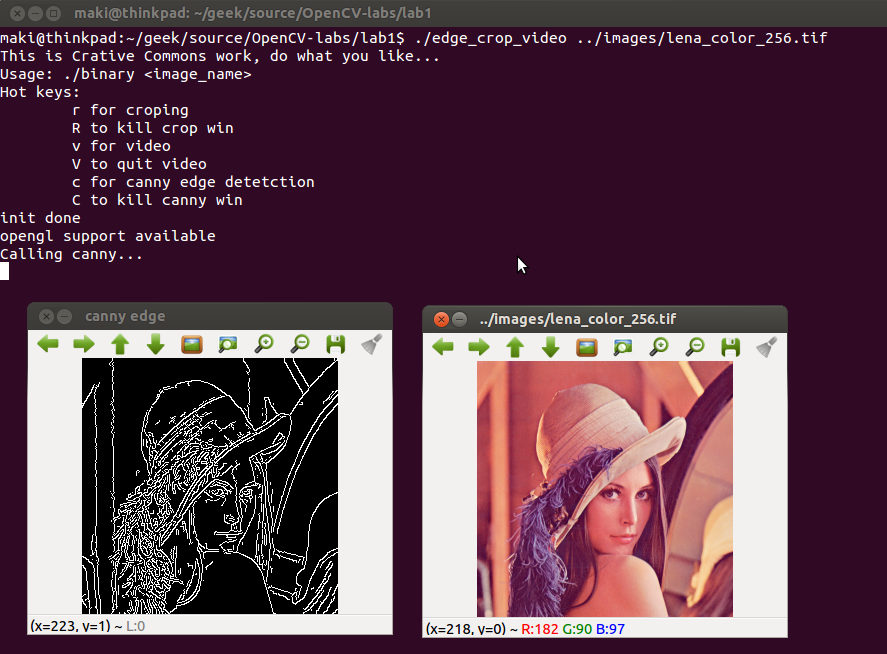
\includegraphics[scale=0.4]{images/lab1-01-edge.png}
\caption{Detekcija rubova}
\label{fig:lab1-01-edge}
\end{figure}

\newpage
\subsubsection{Rezanje slike}
Rezanje slike (engl. \textit{cropping}) je implementirano kroz poziv par
funkcija. Pritiskom na tipku \textbf{``r''} postavlja se
\textit{setMouseCallback} (funkcija koja konstantno poziva drugu
funkciju u slučaju micanja miša ili pritiska tipke) na funkciju
\textit{onMouse}. Funkciji \textit{onMouse} se također kroz
\textit{setMouseCallback} predaje i slika nad kojom je definiran
\textit{callback}.
\\

\begin{lstlisting}[language=C,caption={Rezanje slike}]
void onMouse( int event, int x, int y, int flags, void* param ) {
    Mat& image = *(Mat*) param;
    switch( event ) {
        case CV_EVENT_LBUTTONDOWN:
            drawing_box = true;
            box = Rect(x, y, 0, 0);
            break;
        case CV_EVENT_MOUSEMOVE: 
            if( drawing_box ) {
                box.width = x-box.x;
                box.height = y-box.y;
            } break;
        case CV_EVENT_LBUTTONUP: 
            drawing_box = false;
            if( box.width<0 ) {
                box.x+=box.width;
                box.width *= -1;
            }
            if( box.height<0 ) {
                box.y+=box.height;
                box.height*=-1;
            }
            draw_box( image, box );
            crop_image( image, box);
            break; } } 
void draw_box( Mat& img, Rect rect ){
    rectangle( img, rect.tl(), rect.br(), Scalar(0,0,255));
}
void crop_image( Mat& img, Rect rect ){
    Mat imgRoi = img(rect);
    namedWindow( "ImgROI", CV_WINDOW_AUTOSIZE );
    imshow( "ImgROI", imgRoi );
}
\end{lstlisting}

\begin{figure}[h]
\centering
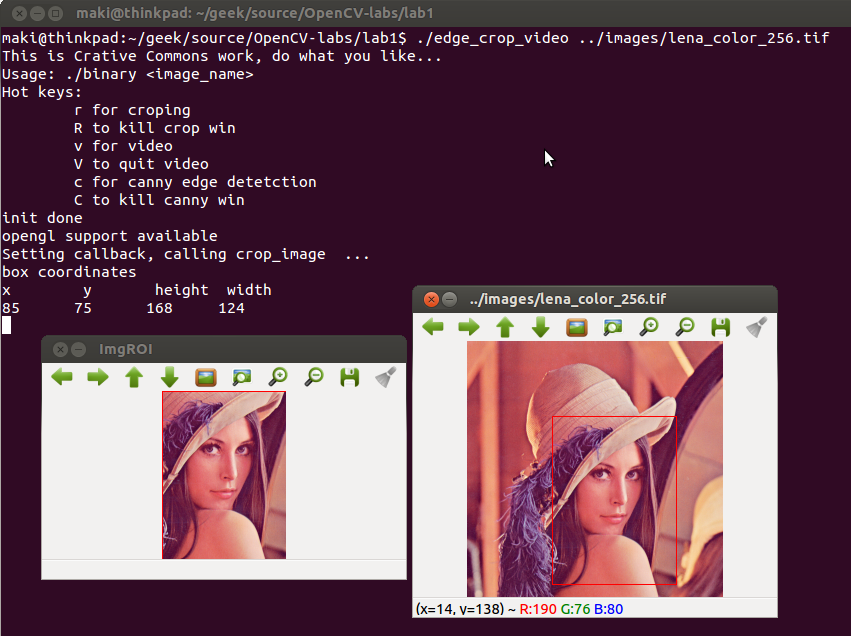
\includegraphics[scale=0.4]{images/lab1-02-crop.png}
\caption{Rezanje slike}
\label{fig:lab1-02-crop}
\end{figure}

\newpage
\subsubsection{Učitavanje videa}
Učitavanje videa ili kamere se događa nakon pritiska tipke
\textbf{``v''}. Time pozivamo funkciju \textit{init\_camera} koja
stvori objekt tipa \textit{VideoCapture}. Objekt prvo pokušu učitat
kameru ako ne uspije provjerava \textit{argv[2]} za drugim izvorom
kamere ili videa. Nakon toga u beskonačnoj petlji objekta se izvlači 
frame po frame i prikazuje u prozoru \textit{``camera``}.
\\
\begin{lstlisting}[language=C,caption={Učitavanje videa}]
void init_camera(){
    cout << "Starting camera mode... \n";
    VideoCapture cap(0);
    if( !cap.isOpened() ){
        cout << "isprobavam argv2 " 
            << global_argv[2] << endl;
        cap.open( global_argv[2] );
        if( !cap.isOpened() ){
            cerr << "fail i preko argv[2] \n"; 
            } 
        }
    while( 1 ){
        cap >> frame;
        if(!frame.data) break;
        namedWindow( "camera", CV_WINDOW_AUTOSIZE );
        imshow( "camera", frame );
        char c = waitKey(10);
        if( c == 'V' ){
            destroyWindow("camera");
            break; 
            } 
        } 
    }
\end{lstlisting}


\subsection{Zaključak}


Osnovni zadaci ove vježbe su bili upoznavanje s OpenCV bibliotekom,
podešavanje radne okoline i rješavanje par jednostavnijih zadataka.
Inicijalno podešavanje radne okoline je bitan zadatak jer o njemu ovisi
izvedba ove i budućih vježbi.
S OpenCV bibliotekom smo se upoznali kroz rješavanje zadataka.
Pisanje jednostavnog programa za detektiranje rubova na slici nam je
pružilo uvid u deklariranje \textit{Mat} varijabli za spremanje slika,
pozivanje OpenCV funkcija i prikazivanje tih slika.
Rješavanje problema rezanja slike nam je omogućilo upoznavanje s
\textit{mouseCallback} funkcijom koja je sastavni dio većine grafičkih
programa. Njeno razumjevanje je ključan dio za pisanje programa koji traže
interakciju s korisnikom. Osim toga naučili korisiti funkciju
\textit{rectangle} za crtanje pravokutnika na slici i definirati regiju
intersa na slici. 
Zadnji dio zadatka se odnosio na učitavanje videa. Osnovna stvar je bila
shvatiti kako \textit{VideoCapture} objekt funkcionira, te koje njegove
metode možemo korisiti.
Svi ovi zadaci su okosnice drugi programa. Detekcija rubova na slici s
kamere se može korisiti u programu koji detektira pokret.
Rezanje slike je poželjna funkcija svakog preglednika slika.



\section{Vježba 2: Metoda podudaranja susjedstva piksela s modelom}

\subsection{Opis vježbe}
Učitati zadanu sliku na kojoj piše neki tekst. Mišem označiti
(kvadratićem zaokružiti) jedno slovo u tekstu na slici. Primjenom metode
podudaranja susjedstva piksela s modelom (engl. \textit{Template
Matching} potrebno je odrediti i označiti (kvadratićem zaokružiti) sva
slična (\textbf{ista}) slova poput označenog slova.

\subsection{Objašnjenje programa}

\subsubsection{Kontrola programa}

Prilikom pokretanja programa iz komandne linije potrebno je 
predati programu putanju do slike (argv[1]) u protivnom se program 
nece pokrenuti. \\

\begin{lstlisting}[language=bash,caption={Pokretanje programa iz
    komandne linije}]
$ ./template_matching ../images/tm-quick.png
\end{lstlisting}

Nakon pokretanja programa u ispisu komandne linije stoji da odaberemo
``t'' za pokretnje template matching-a. Međutim prije toga je prvo
potrebno odredit model odabirom slova ``r'' te nakon toga. Sada možemo
pritisnut ``t'' te će program izbaciti rezultate podudaranja susjedstva
piksel s modelom te označiti slične modele.
\\

\begin{lstlisting}[language=C,caption={Kontrola programa tipkovnicom}]
while (1){
    char c = waitKey(10);
    switch(c) {
        case 'r':
            cout << "Setting callback, calling cropImage  ...\n";
            setMouseCallback(imageName, onMouse, (void*)&loaded_img);
            break;
        case 't':
            if(!croped_roi.data){
                cout << "nisi cropao nista" << endl;
                break; }
            matchTemplateTrackbar( );
            break;
            } }
\end{lstlisting}

\subsubsection{Metoda podudaranje susjedstva piksela s modelom}
Kao što samo ime metode kaže uspoređuje se matrica modela \textbf{T}
(engl. \textit{template}) s matricom slike \textbf{I} na način da
model klizi preko slike. Nad svakim pikselom iz modela izvodi se
matematička funkcija. Funkcija vraća sličnost modela i uspoređenog
dijela slike. Tu vrijednost funkcija zapisuje u rezultantn matricu
\textbf{R}. Opisanu radnju izvršavamo pozivom funkcije
\textit{cv::matchTemplate()}. U toj funkciji je impelementirano šest
matematičkih metoda za pronalazak sličnosti. Svaku od njih se može
isprobati pomicanjem klizača. Nakon dobivanja rezultantne matrice
slijedi pronalazak pozicija piksela koji imaju najveću sličnost modela i
slike. To se možemo odraditi na više načina. Primjerice možemo korisitit 
funkciju \textit{cv::minMaxLoc()}. Ona nam vrati poziciju piksela s najvećom i
najmanjom vrijdnosti. Ta metoda je ograničena na vraćanje samo jednog 
sličnog rezultata. Drugi način je da nad normaliziranom rezultatnom
matricom (vrijdnosti prikazna brojevim između 0 i 1), pustimo funkciju
praga i time odbacimo slabe rezultate. Nakon toga prođemo kroz
matricu i prikažemo sve slične rezultate. Ova metoda je ograničena na
matematičke metode koje se mogu normalizirati.
\\
\begin{lstlisting}[language=C,caption={Podudaranje susjedstva piksela s
    modelom}]
void matchTemplateTrackbar( ){
    namedWindow( "source", CV_WINDOW_AUTOSIZE );
    namedWindow( "result", CV_WINDOW_AUTOSIZE );
    char* trackbar_label = "Method: \n 0: SQDIFF \n 1: SQDIFF NORMED \n 2: TM CCORR \n 3: TM CCORR NORMED \n 4: TM COEFF \n 5: TM COEFF NORMED";
    createTrackbar( trackbar_label, "source" , &match_method, max_Trackbar, matchTemplateOnCrop );
    matchTemplateOnCrop( 0, 0 );
}
void matchTemplateOnCrop( int, void* ){
    Mat source_img;
    loaded_img.copyTo( source_img );
    croped_roi.copyTo( templ_img );
    Mat gsource_img, gtempl_img;
    cv::cvtColor(source_img, gsource_img, CV_BGR2GRAY);
    cv::cvtColor(templ_img, gtempl_img, CV_BGR2GRAY);
    /// Create the result matrix
    int result_cols =  source_img.cols - templ_img.cols + 1;
    int result_rows = source_img.rows - templ_img.rows + 1;   
    result_img.create( result_rows, result_cols, CV_32FC1 );
    /// Do the Matching and Normalize
    matchTemplate( gsource_img, gtempl_img, result_img, match_method);
    normalize( result_img, result_img, 0, 1., NORM_MINMAX, -1, Mat() );
    // Remove non matching results with tresholding
    threshold( result_img, result_img, 0.8, 1., THRESH_BINARY);
    // Localizing the best match with minMaxLoc
    // Used only for testing purpose
    double minVal; double maxVal; double threshold=0.8;
    Point minLoc; Point maxLoc; Point matchLoc;
    minMaxLoc( result_img, &minVal, &maxVal, &minLoc, &maxLoc);
    rectangle( source_img, maxLoc, Point( maxLoc.x + templ_img.cols , maxLoc.y + templ_img.rows ), Scalar(0,0,255) ); 
    int x,y;
    // Go througe rows
    for (y = 1; y < result_img.rows -1; y++) {
        for (x = 1; x < result_img.cols -1; x++) {
            if (result_img.at<float>(y,x) > 0) {
                cout << y << "," << x << " = " << result_img.at<float>(y,x) << endl; 
                rectangle( source_img, Point(x,y), Point (x+templ_img.cols, y+templ_img.rows), Scalar(0,255,0));  
            } } }
    imshow( "source", source_img );
    imshow( "result", result_img);
}
\end{lstlisting}

\begin{figure}[h]
\centering
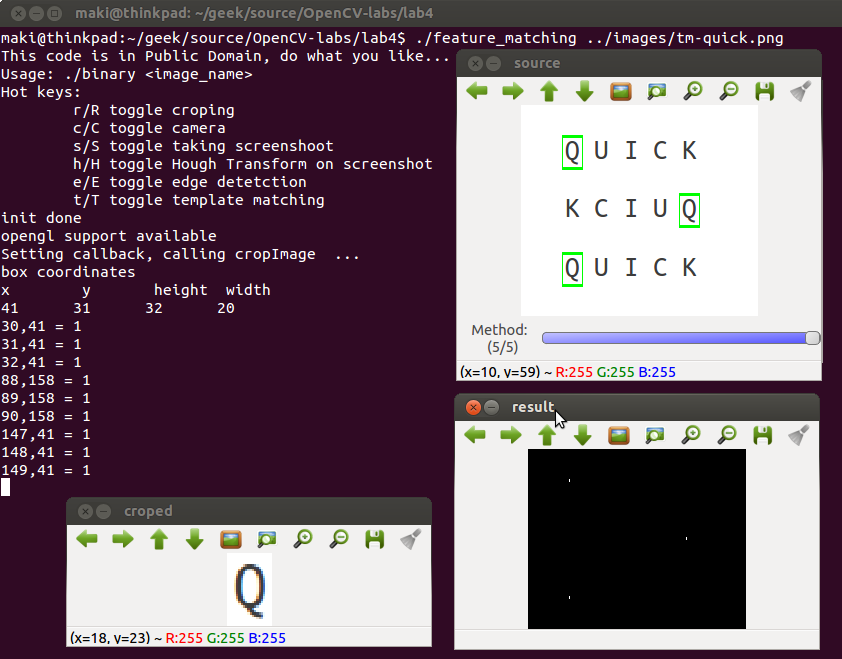
\includegraphics[scale=0.4]{images/lab2-01-tm.png}
\caption{Detekcija rubova}
\label{fig:lab2-01-tm}
\end{figure}

\subsection{Zaključak}
Glavni zadatak ove vježbe je bio pronalazk istih slova i njihova
označavanje.
Rješavanje tog problema zahtjevalo je razumjevanje rada
\textit{cv::matchTemplate()} funkcije i njenog korištenja rezultantne
matrice. Zatim je bilo bitno razumjeti kako je spremaljena rezultatna 
matrica u memoriji kako bi mogli pronaći lokacije svih sličnih modela.
Program daje dobre rezultate samo kod matematičkih funkcija koje se mogu
normalizirati, te je to područje koje se može unaprijediti.
Logika ovog programa je okosnica većine programa za optičko
prepoznavanje znakova (engl. \textit{optical character recognition}, a
postoje i mnoge druge primjene ove metode.


\section{Vježba 3: Houghova transformacija}

\subsection{Opis vježbe}
Potrebno je pomoću, prethodno kalibrirane, web kamere uslikati objekt
kvadratnog oblika koji je postavljen na milimetarskom papiru na stolu.
Primjenom Houghove transformacije (HT) treba odrediti parametre \(\rho
\) i \( \theta \)najdominantnijeg pravca, koji odgovara jednom od rubova objekta
na slici. Pod najdominantnijim pravcem podrazumijeva se pravac kojem
pripada najveći broj 'glasova' u akumulacijskoj ravnini. Implementacija
HT u biblioteci OpenCV vraća popis detektiranih pravaca koji su
razvrstani prema broju 'glasova' počevši od najdominantnijeg. Primjenom
odgovarajuće transformacije, odrediti \(\rho i \theta \)tog pravca u
koordinatnom sustavu milimetarskog papira. Provjeriti koliko je
odstupanje dobivenog pravca od stvarnog (odgovarajućeg) ruba objekta.

\subsection{Kalibracija kamere}
Cijenovna prihvatljivosti web kamera ima svoju negativnu stranu, a to je
značajna distorzija. Postoji radijalni efekt (\textit{fisheye}) i
tangencijalna distorzija (leće kamere nisu u savršeno paralelene s
ravninom slikanja). Zato kalibracijom kamere možemo rješiti te
nedostatke. Isto tako kalibracijom možemo odrediti vezu između piksela i
milimetara.

Za kalibraciju smo koristili program koji se kompajlira prilikom
kompajliranja OpenCV biblioteke. Pomoću njega smo dobili koeficiente
distorzije i matricu kamere. Te podatke program dobije računanjem
jednostavnih geometrijskih jednadžbi nad primjerom crno bijele šahovske ploče.

\begin{figure}[h]
\centering
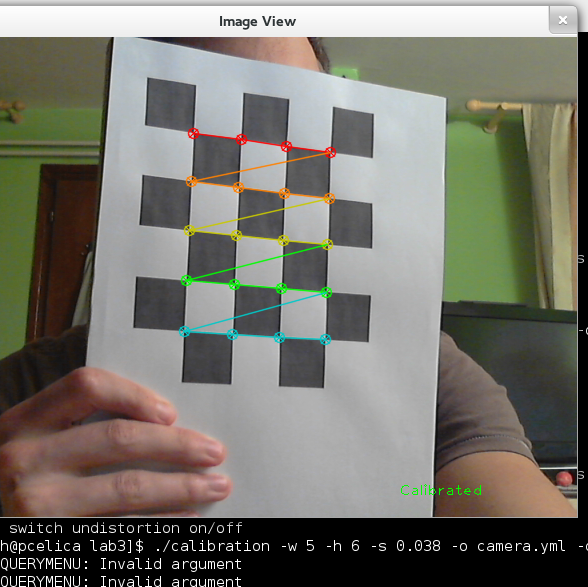
\includegraphics[scale=0.37]{images/lab3-01-calib.png}
\caption{Kalibracija kamere}
\label{fig:lab3-01-calib}
\end{figure}

\newpage
\subsection{Objašnjenje programa}

\subsubsection{Kontrola programa}

Prilikom pokretanja programa iz komandne linije potrebno je 
predati programu putanju do slike (argv[1]) ako nad njom želimo provesit
HT ili možemo uzeti sliku putem kamere.
\\
\begin{lstlisting}[language=C,caption={Kontrola programa tipkovnicom}]
while (1){
    char c = waitKey(10);
    switch(c) {
            case 'c':
                initCamera ();
                break;
            case 'h':
                if (!imageTaken) {
                    if (pointSelected) {
                        cannyEdge (loadedImg, ssBox);
                        cout << "Points?!1\n";
                    }
                    setMouseCallback (imageName, getPoints, 0);
                    cout << "No data from camera. Using argv[1] or \ default image\n";
                }
                else { 
                cannyEdge (ssImg, ssBox);
                }
                break;
            case 'H':
                callHoughTransform ();
                destroyWindow ("snapshot");
                break;
\end{lstlisting}

\begin{itemize}
    \item Pokrenut kameru pritiskom na ``c''
    \item Uslikati objekt na milimetarskom papiru s ``i''
    \item Označiti (klikom) četiri ugla milimetarskog papira
    \item Ugasiti kameru pritsikom na ``C''
    \item Pokrenuti filtiranje slike pritiskom na ``h''
    \item Pozvati houghovu transformaciju pritiskom na ``H''
\end{itemize}


\subsubsection{Houghova transformacija}
Detektiranje linija i određivanje  \(\rho \) i \( \theta \) u
koordinatnom sustavu milimetarskog papira je implementirano u funkciji
\textit{callHoughTransform()}.

\begin{lstlisting}[language=C,caption={Racunanje parametra ro i theta}]
int callHoughTransform ()
{
    /*
     * Find lines in edge point image using Hough Transform
     * HT is operating in polar coordinte system so our lines are
     * represented with: 
     * rho - vector from origin of c.s to line (perpendicular to line) 
     * theta - angle form positive x axis to rho (range -90-90)
     */
    vector<Vec2f> lines;
    HoughLines (cannyOut, lines, 1, CV_PI/180, 100, 0, 0);
    // cout << "Lines = " << Mat( lines ) << endl;
    if (lines.empty()) {
        cout << "HT didn't find lines, run edge with more details\n";
        return -1;
    }
    float rho, rhoRoi, theta;
    rhoRoi = lines[0][0];
    theta = lines[0][1];
    // Computes rho in image c.s.
    rho = rhoRoi + pt1.x * cos(theta) + pt1.y * sin(theta);
    // Read calibration parameters
    FileStorage fs ("../lab3/calib/cam-c270.xml", FileStorage::READ);
    // Intrinsics/projection matrix with fx,fy,u,v intrinsics camera
    // parameters for unit conversion
    Mat intrinsics (3, 3, CV_32F); 
    fs ["camera_matrix"] >> intrinsics; 
    // Distortion matrix with k1,k2,p1,p2,k3 distortion coefficients
    // for correcting cameras radial and tangential distortion
    Mat distortion (5, 1, CV_32F);
    fs ["distortion_coefficients"] >> distortion; 
    // Dimension's of graph paper in mm
    vector<Point3f> objectPoints (4);
    objectPoints[0] = Point3f (0, 0, 0);
    objectPoints[1] = Point3f (0, 265, 0);
    objectPoints[2] = Point3f (170, 0, 0);
    objectPoints[3] = Point3f (170, 265, 0);
    // Rotation vector output from solvePnP
    Mat rvec (1, 3, CV_32F);
    // Translation vetor - descrabise position of object c.s.     
    // in regards to camera c.s
    Mat tvec (1, 3, CV_32F);
    // Estimate object position from 3D-2D point correspondences.
    solvePnP (Mat (objectPoints), Mat (imagePoints), intrinsics,
            distortion, rvec, tvec, false);
    // Rotation matrix - describes orientation of object c.s. 
    // in regards to camera c.s
    Mat R (3, 3, CV_32F);
    // Converts rotation vector to rotation matrix
    Rodrigues (rvec, R);
    //cout << "R = " << R <<  endl;
    // A matrix store unit converted rotation matrix
    Mat A (3, 3, CV_32F);
    A = intrinsics * R; 
    // B vector stores crorrected translation vector
    Mat B (3, 1, CV_32F);
    B = intrinsics * tvec;
    double lambdaX, lambdaY, lambdaRo, rhoCrtano, thetaCrtano;
    lambdaX = A.at<double>(0,0) * cos(theta) + A.at<double>(1,0) *
        sin(theta) - rho * (A.at<double>(2,0));
    lambdaY = A.at<double>(0,1) * cos(theta) + A.at<double>(1,1) *
        sin(theta) - rho * (A.at<double>(2,1));
    lambdaRo = rho * (B.at<double>(2)) - B.at<double>(0) * 
        cos(theta) - B.at<double>(1) * sin(theta); 
    thetaCrtano = atan2 (lambdaY, lambdaX);
    rhoCrtano = lambdaRo / sqrt (lambdaX * lambdaX + lambdaY * lambdaY);
    cout << "Theta = " << thetaCrtano*180/CV_PI "degres" << endl;
    cout << "Rho = " << rhoCrtano << "mm" << endl;
    return 0;
}
\end{lstlisting}

\newpage
\begin{figure}
\centering
\begin{minipage}{.5\textwidth}
  \centering
  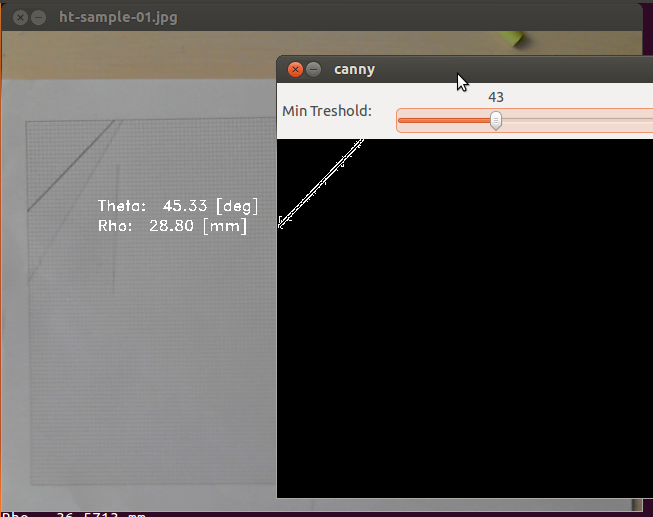
\includegraphics[width=.9\linewidth]{images/lab3-sample-01.png}
  \caption{A figure}
  \label{fig:test1}
\end{minipage}%
\begin{minipage}{.5\textwidth}
  \centering
  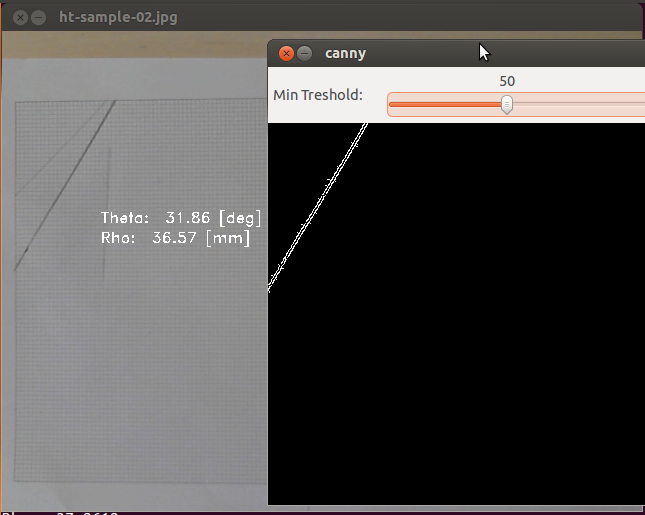
\includegraphics[width=.9\linewidth]{images/lab3-sample-02.png}
  \caption{Another figure}
  \label{fig:test2}
\end{minipage}
\end{figure}

\begin{figure}[h]
\centering
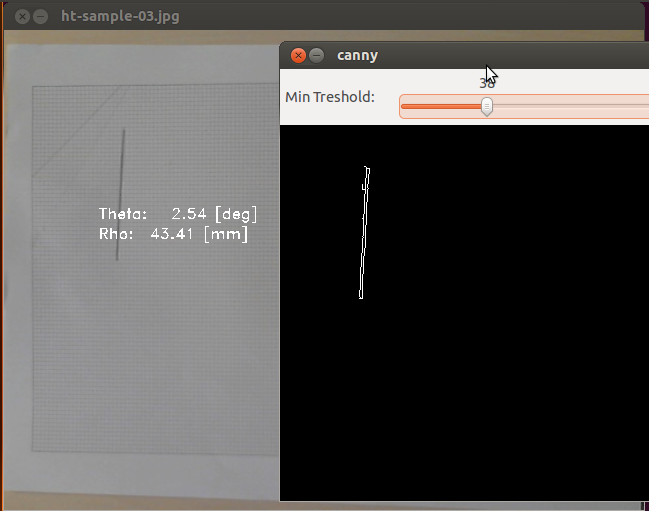
\includegraphics[scale=0.32]{images/lab3-sample-03.png}
\caption{Houghova transformacija}
\label{fig:lab3-sample-03}
\end{figure}

\subsection{Rezultati}

\begin{center}
\centering
\begin{tabular}
{ l || c | c | p{1.6 cm} | p{1.6 cm}  }
{uzorak}  & {\(\theta\) $[mm]$ } & {\(\rho \) $[mm]$} & {izmjerena \(\theta\) $[mm]$} & {izmjeren \(\rho\) $[mm]$} \\ \hline
ht-sample-01 & 45.33 & 28.80 & 45 & 30 \\ \hline
ht-sample-02 & 31.86 & 36.57 & 32 & 39 \\ \hline
ht-sample-03 & 2.54 & 43.41 & 3 & 44 \\ 
\end{tabular}
\end{center}

\newpage
\subsection{Zaključak}



\section{Vježba 4: SURF}

\subsection{Opis vježbe}
Izraditi 2D model nekog objekta na temelju slike tog objekta snimljenog
kamerom. Razmatrani model predstavlja skup 2D točaka detektiranih
SURF-metodom kojima su pridruženi lokalni deskriptori. Potrebno je
raspoznati objekt na drugoj slici koja je također snimljena kamerom, ali
iz drugog položaja.  
\\
\begin{lstlisting}[language=bash,caption={Pokretanje programa iz
    komandne linije}]
$ ./feature_matching ../images/sm-object.jpg ../images/sm-scene.jpg 
\end{lstlisting}

\subsection{Objašnjenje programa}

\subsubsection{Kontrola programa}

Prilikom pokretanja programa iz komandne linije potrebno je 
predati programu putanju do slike objekta (argv[1]) i putanju do slike
scene (argv[2]). 
\\

\begin{lstlisting}[language=C,caption={Kontrola programa tipkovnicom}]
while (1){
    char c = waitKey(10);
    switch(c) {
            case 's':
                surfFlannMatcher ();
                break;
\end{lstlisting}

\newpage
\subsubsection{SURF}

\begin{lstlisting}[language=C,caption={Detekcija objekta na drugoj
    slici}]
void surfFlannMatcher ()
{
    Mat imgObject = imread (globalArgv[1], CV_LOAD_IMAGE_GRAYSCALE);
    Mat imgScene = imread (globalArgv[2], CV_LOAD_IMAGE_GRAYSCALE);
    if (!imgObject.data || !imgScene.data) { 
      cout<< "Error reading images " << endl; 
      return; 
    }

    // Threshold for the keypoint detector. Only features, 
    // whose hessian is larger than minHessian are 
    // retained by the detector. Therefore, the larger the
    // value, the less keypoints you will get.
    int minHessian = 400;
    // Detect the keypoints using SURF Detector
    SurfFeatureDetector detector(minHessian);
    vector<KeyPoint> keypointsObject, keypointsScene;

    // Detection of object and scene keypoints (location, 
    // diameter of the meaningful keypoint neighborhood)
    detector.detect (imgObject, keypointsObject);
    detector.detect (imgScene, keypointsScene);
    cout << "Number of keypoints in object: " << 
        keypointsObject.size() << endl;
    cout << "Number of keypoints in scene: " << 
        keypointsScene.size() << endl;

    // Calculate descriptors (feature vectors)
    // on detected keypoints
    SurfDescriptorExtractor extractor;
    Mat descriptorsObject, descriptorsScene;
    extractor.compute (imgObject, keypointsObject, descriptorsObject);
    extractor.compute (imgScene, keypointsScene, descriptorsScene);

    // Matching descriptor vectors using FLANN matcher
    // Fast approximate nearest neighbor
    FlannBasedMatcher matcher;
    // DMatch - Class for matching keypoint descriptors
    vector<DMatch> matches;
    matcher.match (descriptorsObject, descriptorsScene, matches);

    double maxDist = 0; double minDist = 100;
    // Quick calculation of max and min distances between keypoints
    for( int i = 0; i < descriptorsObject.rows; i++ ) { 
        double dist = matches[i].distance;
        if( dist < minDist ) minDist = dist;
        if( dist > maxDist ) maxDist = dist;
    }
    // Class for matching keypoint descriptors: 
    // query descriptor index, train descriptor index, 
    // train image index, and distance between descriptors.
    vector<DMatch> goodMatches;
    // Draw only "good" matches (i.e. whose distance is 
    // less than 3*minDist )
    for( int i = 0; i < descriptorsObject.rows; i++ )
    { if( matches[i].distance < 3*minDist )
     { goodMatches.push_back( matches[i]); }
    }

    Mat imgMatches;
    // Draws only paired keypoints with random colors
    drawMatches (imgObject, keypointsObject, imgScene, keypointsScene,
               goodMatches, imgMatches, Scalar::all(-1), 
               Scalar::all(-1), vector<char>(), 
               DrawMatchesFlags::NOT_DRAW_SINGLE_POINTS);

    // Localize the object
    vector<Point2f> obj;
    vector<Point2f> scene;
    for (int i = 0; i < goodMatches.size(); i++) {
    // Get the keypoints location from the good matches
    obj.push_back (keypointsObject[ goodMatches[i].queryIdx ].pt);
    scene.push_back (keypointsScene[ goodMatches[i].trainIdx ].pt);
    }
    // Finds a perspective transformation between two planes.
    // Using RANSAC method
    Mat H = findHomography (obj, scene, CV_RANSAC);

    // Get the corners from the image1 (the object to be "detected")
    vector<Point2f> objCorners(4);
    objCorners[0] = cvPoint (0,0); 
    objCorners[1] = cvPoint (imgObject.cols, 0);
    objCorners[2] = cvPoint (imgObject.cols, imgObject.rows); 
    objCorners[3] = cvPoint (0, imgObject.rows);
    vector<Point2f> sceneCorners(4);

    // Perfom perspective transform 
    perspectiveTransform (objCorners, sceneCorners, H);
    // Draw lines between the corners 
    // (the mapped object in the scene - image2)
    line (imgMatches, sceneCorners[0] + Point2f (imgObject.cols, 0), 
            sceneCorners[1] + Point2f (imgObject.cols, 0), 
            Scalar(0, 255, 0), 4);
    line (imgMatches, sceneCorners[1] + Point2f (imgObject.cols, 0), 
            sceneCorners[2] + Point2f (imgObject.cols, 0), 
            Scalar( 0, 255, 0), 4);
    line (imgMatches, sceneCorners[2] + Point2f (imgObject.cols, 0), 
            sceneCorners[3] + Point2f (imgObject.cols, 0), 
            Scalar( 0, 255, 0), 4);
    line (imgMatches, sceneCorners[3] + Point2f (imgObject.cols, 0), 
            sceneCorners[0] + Point2f (imgObject.cols, 0), 
            Scalar( 0, 255, 0), 4);
    // Show detected matches
    imshow ("Good Matches & Object detection", imgMatches);
    waitKey(0);
}
\end{lstlisting}

\begin{figure}[h]
\centering
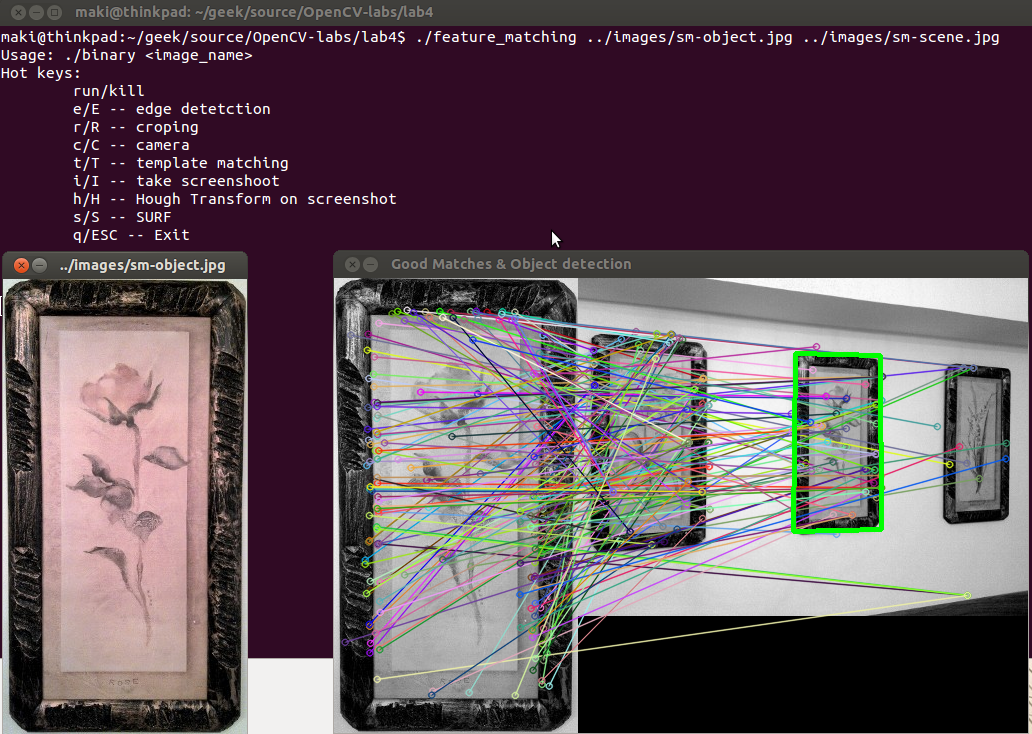
\includegraphics[scale=0.42]{images/lab4-surf-01.png}
\caption{SURF - pronalazak objekta u sceni}
\label{fig:lab4-surf-01}
\end{figure}

\newpage
\subsection{Zaključak}


%\include{05_peta}

\end{document}

